%-------------------------
% Resume in Latex
% Author : Jake Gutierrez
% Based off of: https://github.com/sb2nov/resume
% License : MIT
%------------------------

\documentclass[letterpaper,11pt]{article}

\usepackage{latexsym}
\usepackage[empty]{fullpage}
\usepackage{titlesec}
\usepackage{marvosym}
\usepackage[usenames,dvipsnames]{color}
\usepackage{verbatim}
\usepackage{enumitem}
\usepackage[hidelinks]{hyperref}
\usepackage{fancyhdr}
\usepackage[english]{babel}
\usepackage{tabularx}
\usepackage{fontawesome5}
\usepackage{multicol}
\usepackage{wasysym}
\usepackage{lastpage}


\usepackage{tikz}
\usepackage{graphicx}

\setlength{\multicolsep}{-3.0pt}
\setlength{\columnsep}{-1pt}
\input{glyphtounicode}
\usepackage{fontawesome5}

\newcommand{\portfoliosymbol}{\faFolderOpen\hspace{-.1em}\faBriefcase}

\pagenumbering{arabic}



%----------FONT OPTIONS----------
% sans-serif
% \usepackage[sfdefault]{FiraSans}
% \usepackage[sfdefault]{roboto}
% \usepackage[sfdefault]{noto-sans}
% \usepackage[default]{sourcesanspro}

% serif
% \usepackage{CormorantGaramond}
% \usepackage{charter}


\pagestyle{fancy}
\fancyhf{} % clear all header and footer fields
\fancyfoot{}
\renewcommand{\headrulewidth}{0pt}
\renewcommand{\footrulewidth}{0pt}

% Adjust margins
\addtolength{\oddsidemargin}{-0.6in}
\addtolength{\evensidemargin}{-0.5in}
\addtolength{\textwidth}{1.19in}
\addtolength{\topmargin}{-.7in}
\addtolength{\textheight}{1.4in}

\urlstyle{same}

\raggedbottom
\raggedright
\setlength{\tabcolsep}{0in}

% Sections formatting
\titleformat{\section}{
  \vspace{-4pt}\scshape\raggedright\large\bfseries
}{}{0em}{}[\color{black}\titlerule \vspace{-5pt}]

% Ensure that generate pdf is machine readable/ATS parsable
\pdfgentounicode=1

%-------------------------
% Custom commands
\newcommand{\resumeItem}[1]{
  \item\small{
    {#1 \vspace{-2pt}}
  }
}

\newcommand{\classesList}[4]{
    \item\small{
        {#1 #2 #3 #4 \vspace{-2pt}}
  }
}

\newcommand{\resumeSubheading}[4]{
  \vspace{-2pt}\item
    \begin{tabular*}{1.0\textwidth}[t]{l@{\extracolsep{\fill}}r}
      \textbf{#1} & \textbf{\small #2} \\
      \textit{\small#3} & \textit{\small #4} \\
    \end{tabular*}\vspace{-7pt}
}

\newcommand{\resumeSubSubheading}[2]{
    \item
    \begin{tabular*}{0.97\textwidth}{l@{\extracolsep{\fill}}r}
      \textit{\small#1} & \textit{\small #2} \\
    \end{tabular*}\vspace{-7pt}
}

\newcommand{\resumeProjectHeading}[2]{
    \item
    \begin{tabular*}{1.001\textwidth}{l@{\extracolsep{\fill}}r}
      \small#1 & \textbf{\small #2}\\
    \end{tabular*}\vspace{-7pt}
}

\newcommand{\resumeSubItem}[1]{\resumeItem{#1}\vspace{-4pt}}

\renewcommand\labelitemi{$\vcenter{\hbox{\tiny$\bullet$}}$}
\renewcommand\labelitemii{$\vcenter{\hbox{\tiny$\bullet$}}$}

\newcommand{\resumeSubHeadingListStart}{\begin{itemize}[leftmargin=0.0in, label={}]}
\newcommand{\resumeSubHeadingListEnd}{\end{itemize}}
\newcommand{\resumeItemListStart}{\begin{itemize}}
\newcommand{\resumeItemListEnd}{\end{itemize}\vspace{-5pt}}

%-------------------------------------------
%%%%%%  RESUME STARTS HERE  %%%%%%%%%%%%%%%%%%%%%%%%%%%%


\begin{document}

%----------HEADING----------
% \begin{tabular*}{\textwidth}{l@{\extracolsep{\fill}}r}
%   \textbf{\href{http://sourabhbajaj.com/}{\Large Sourabh Bajaj}} & Email : \href{mailto:sourabh@sourabhbajaj.com}{sourabh@sourabhbajaj.com}\\
%   \href{http://sourabhbajaj.com/}{http://www.sourabhbajaj.com} & Mobile : +1-123-456-7890 \\
% \end{tabular*}
\parbox{3.0cm}{%

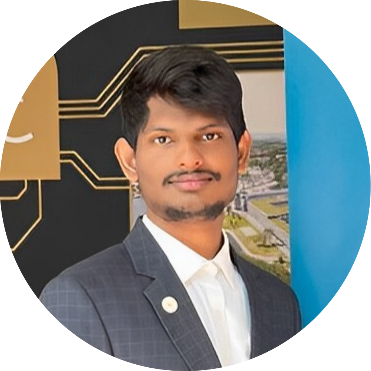
\includegraphics[width=2.7cm,clip]{images/resume_pic_m.png}}
}
\parbox{\dimexpr\linewidth-3.8cm\relax}{
\vspace{-20pt}
\begin{tabularx}{\linewidth}{L r} \\
    {\Huge \scshape  Venkata Sai Yakkshit Reddy Asodi}~
    \href{https://www.cedzlabs.com/yakkshit}{\vspace{1pt}}\\
      Kungsmarkvågen 69 37144. \\ \vspace{1pt}
     \small \raisebox{-0.1\height}\faPhone\ +46 0793550685 ~ \href{mailto:saiyakkshit2001@gmail.com}{\raisebox{-0.2\height}\faEnvelope\  {saiyakkshit2001@gmail.com}} ~ 
    \href{https://linkedin.com/in/yakkshit/}{\raisebox{-0.2\height}\faLinkedin\ {yakkshit}}  ~
    \href{https://yakkshit.com/}{\raisebox{-0.2\height}\faGlobe\ {yakkshit.com}}  ~
    \href{https://github.com/yakkshit}{\raisebox{-0.2\height}\faGithub{ saiyakkshit}}
    \vspace{-8pt}
    
\end{tabularx}
}




\vspace{-10pt}
%-----------EDUCATION-----------
\section{Education Details  \faGraduationCap   }


% \hfill \textbf{\LARGE 
%  \raisebox{9pt} {Software Developer}}
 
  \resumeSubHeadingListStart
    \resumeSubheading
      {Blekinge Institute of Technology}{Sep. 2022 -- June. 2023}
      {Bachelor of Science in Computer Science}{\faMapMarker Valhallavägen 1, 371 41 Karlskrona.}
  \resumeSubHeadingListEnd
    \vspace{-15pt}
  \resumeSubHeadingListStart
    \resumeSubheading
      {University College Of Engineering Jntuk}{Aug. 2019 -- Jun. 2022}
      {Bachelor of Science in Computer Science}{\faMapMarker Kakinada, AndhraPradesh, India 533003.}
  \resumeSubHeadingListEnd
\vspace{-22pt}
%-----------------------------------
\href{https://www.yakkshit.com/#details}{\section{Summary \faLink}
I am a \textbf{Software Engineer} with a passion for building high-quality software. I have experience in \textbf{full-stack development} and have contributed to the product lifecycle, from requirements analysis to deployment. I have a strong understanding of authentication and authorization, and I effectively manage monitoring and logs using tools such as Prometheus, Jenkins, Grafana, Azure CLI. I have hands-on experience with \textbf{CI/CD, DevOps, infrastructure as code, and GitHub}. I am an agile thinker with a passion for continuous learning, and I am able to mentor and guide junior team members.}



% As a tech enthusiast currently pursuing a Bachelor's degree in Computers at the Blekinge Institute of Technology, I am equipped with a strong foundation in computer science and a passion for leveraging technology to drive innovation. With a focus on Python, Java, and AI, I have completed certifications such as MTA-Python and Java, AI-Intern, and GCP Cloud Carrier Path. My practical experience includes developing a Google Assistant using Google Cloud services and APIs, utilizing RESTful APIs and JSON for communication, and deploying apps on Google Home and Google Hub devices. By combining my technical skills with hands-on experience in AI engineering and Android app testing, I have gained proficiency in TensorFlow, OpenCV, and automation testing using tools like Appium. I am adept at collaborating within a team to enhance user experience and ensure web security. With a track record of successfully completing projects such as AWS file encryption and Langversation, an end-to-end encrypted multilingual chat-based Android application, I have demonstrated my ability to implement secure systems and leverage technologies like AWS KMS, S3, Firebase, and Kubernetes. Through my coursework and extracurricular involvement, I have developed strong leadership skills, multitasking abilities, and meticulous attention to detail. As I continue to explore emerging technologies like augmented reality and system administration, I am committed to continuous learning and leveraging my expertise to contribute to cutting-edge projects in the field of computer science.


 \vspace{-10pt}


 %-----------EDUCATION-----------

%-----------EXPERIENCE-----------
\section{\href{https://www.linkedin.com/in/yakkshit/}{Professional Experience  \faLink}}
  \resumeSubHeadingListStart
  \resumeSubheading
      {BetaTesting, Inc}{Jan 2023 -- June 2023}
      {Android Application Tester}{\faMapMarker Remote}\\
      \vspace{10pt}
      \textbf{Description:}
      I Have worked as a beta tester for the New App Launcher on Android Phones, identifying and reporting bugs to the development team, and developed problem-solving skills and attention to detail through this experience. I have also learned to work collaboratively with a team to improve user experience and web security.
      \vspace{-10pt}
      \textbf{Responsibilities:}
      \resumeItemListStart
        \resumeItem{Conducted beta testing for new Android app launcher by developing a comprehensive test plan, executing test cases, and identifying/reporting 25+ critical bugs to the development team; reduced the overall bug rate by 40\%.}
        \resumeItem{I have used the following testing methods Functional, Load, Security, Compatibility, Usability, Automated Testing to enhance the performance of the Application.}
        \resumeItem{Utilizing Android Studio as the development environment to visualize and analyze the application and Leveraging performance analysis.}
    \resumeItemListEnd
    \vspace{-3pt}
    \textbf{Environment:}\emph{Android app testing, bug reporting, problem-solving, collaboration, Android Studio, Appium.}
    \vspace{-5pt}

    \resumeSubheading
      {Cedzlabs.com}{May 2021 -- Dec 2022}
      {FullStack Engineer}{\faMapMarker Remote}\\
      \vspace{10pt}
      \textbf{Description : }I was responsible for creating and maintaining both the front-end and back-end components of websites and web applications
as a full-stack engineer at CedzLabs. Working with a range of programming languages and technologies.\\
\textbf{Responsibilities : }
      \vspace{-5pt}
      \resumeItemListStart
        \resumeItem{Utilized a range of programming languages and technologies including HTML, CSS, JavaScript, Node.js, Django, and SQL databases.}
        \resumeItem{Implemented the Django framework to enhance the functionality and interactivity of websites.}
        \resumeItem{Integrated various RESTfulAPIs to enhance the functionality and features of the websites.}
        \resumeItem{Monitored website performance using also the Google search console, Google Analytics, and crashes using Firebase Performance SDK.}\\

      \resumeItemListEnd
\vspace{0.5pt}
\textbf{Environment:}\emph{HTML, CSS, JS, TypeScript, PHP, nodejs, SQL, Django, JSON, ML, Firebase, GCP.}
  


    \resumeSubheading
      {VERZEO.INC}{Aug 2020 -- Mar 2021}
      {AI Engineer Intern}{ \faMapMarker Remote}\\
      \vspace{10pt}
      \textbf{Description : }I developed a Python project that uses computer vision and deep learning to detect face masks and human falls. The project achieved 95\%\ accuracy for face mask detection and 85\%\ accuracy for human fall detection. It can be used in a variety of applications, such as monitoring compliance with COVID-19 safety regulations. This project is a valuable contribution to the field of computer vision.\\

      
\textbf{Responsibilities : }
      \vspace{-5pt}
      \resumeItemListStart
        \resumeItem{Utilized Python, TensorFlow, OpenCV, and deep learning techniques to implement the project, working with a provided dataset.}
        \resumeItem{Integrated the trained model into a real-time face mask detection system using the OpenCV library and its computer vision capabilities.}
        \resumeItem{Conducted comprehensive testing to ensure the precision and reliability of the face mask detection system.}
        \\

      \resumeItemListEnd
\vspace{-3pt}
\textbf{Environment:}\emph{Python, TensorFlow, OpenCV, Keras, Deep learning.}
\vspace{-5pt}
\resumeSubHeadingListEnd

%-----------PROJECTS-----------
\section{\href{https://www.yakkshit.com/#project-1}{Projects} \faLink}
    \vspace{-5pt}
    \resumeSubHeadingListStart
    \resumeProjectHeading          {\textbf{\href{https://github.com/saiyakkshit/Langversation}{Langversation}} $|$ \emph{CI/CD, Android Studio}}{December 2022}\\
          \vspace{6pt}
          \textbf{Description:}
         
          \vspace{-8pt}
          \resumeItemListStart
            \resumeItem{ Langversation is a communication, end‑to‑end encrypted multilingual chat‑based android application which was developed in kotlin.}
            \resumeItem{In the development of user conversation i have used XML as front end and Kotlin for the back end.}
            \resumeItem{For the storage and authentication which was used in the app was done in FirebaseStorage and FirebaseAuthentication.}
            \resumeItem{Ml kit translational API which was used to convert from one language to the other.}
            \resumeItem{The Performance and Crashes of the App was monitered using the Firebase Performance SDK and Firebase Crashlytics SDK.}
          \resumeItemListEnd 
          \textbf{Tools:}\emph{
Kotlin, java, ML kit, Firebase, XML.}
%       \resumeProjectHeading
%       {\textbf{\href{https://review.gerrithub.io/admin/repos/saiyakkshit/py-chess-svg,general}{Deploying an Application using Gerrit}} $|$ \emph{CI/CD, Visual Studio Code.}}{March 2023}\\
%           \vspace{6pt}
%           \textbf{Description:}
%           \vspace{-5pt}
%           \resumeItemListStart
%     \resumeItem{\href{https://review.gerrithub.io/admin/repos/saiyakkshit/py-chess-svg,general}{Implemented Zuul CI with Gerrit Code Review, utilizing Zuul concepts and project gating for efficient code review and integration process}.}
%             \resumeItem{\href{https://review.gerrithub.io/admin/repos/saiyakkshit/py-chess-svg,general}{Developed a Python project integrated with Zuul, incorporating third-party dependencies such as python-chess to generate SVG images based on input moves}.}
%             \resumeItem{\href{https://review.gerrithub.io/admin/repos/saiyakkshit/py-chess-svg,general}{Extended the project with Bazel integration, creating a Python wheel file, performing unit tests, and utilizing Zuul for artifact management and coverage reports.}}
%           \resumeItemListEnd 
%           \textbf{Tools:}\emph{\href{https://review.gerrithub.io/admin/repos/saiyakkshit/py-chess-svg,general}{
% Zuul CI, Gerrit Code Review, Bazel, unit tests, Jtest, coverage reports.}}
        \vspace{-18pt}
          
          \resumeProjectHeading
          {\href{https://yakkshit.com}{\textbf{AWS Hosting Deployment, Monitoring, and Serverless Functions}} $|$ \emph{NextJS, AWS CLI}}{January 2023}\\
          \vspace{6pt}
          \textbf{Description:}
          
          \vspace{-5pt}
          \resumeItemListStart
            \resumeItem{\href{https://yakkshit.com}{Designed and implemented a secure file encryption/decryption system using AWS KMS and S3, with access controls enforced through IAM.}}
            \resumeItem{\href{https://yakkshit.com}{Built and deployed a scalable and efficient website using NextJS, threeJS, and AWS services (S3, Lambda), leveraging GitHub Actions for automated deployment and builds, and monitored website performance using AWS CloudWatch. Additionally, utilized the Storybook component library to enhance the design and development process, and hosted the website on GitHub Pages for easy access and visibility.}}
            \resumeItem{\href{https://yakkshit.com}{Designed and developed a visually appealing and user-friendly UI/UX for my portfolio website using Figma and React, with a component-centric approach that enhances the user experience.}}
          \resumeItemListEnd
          \vspace{-2pt}
          \textbf{Tools:}\emph{ \href{https://yakkshit.com}{AWS KMS, S3, encryption, decryption, unique key, IAM, secure files, web development, Nextjs, React.}}
          \vspace{-18pt}
          \resumeProjectHeading
          {\textbf{\href{https://github.com/saiyakkshit?tab=repositories}{Networking and Firewalls}} $|$ \emph{Bash, Ubuntu}}{November 2022}\\
          \vspace{6pt}
          \textbf{Description:}
           \vspace{-5pt}
          \resumeItemListStart
            \resumeItem{Established communication between networked devices using bash scripting and Ubuntu.}
            \resumeItem{Employed HTTP requests for data transfer and set up firewall rules to ensure secure communication.}
            \resumeItem{Updated firewall rules to establish a secured connection between client and server.}           
          \resumeItemListEnd 
          \textbf{Tools:}\emph{Bash scripting,
Ubuntu OS,
C Programming,
HTTP requests, Network Security,
Firewall rules.}
          \vspace{-18pt}
          % \resumeProjectHeading
          % {\textbf{\href{https://www.cloudskillsboost.google/public_profiles/6bf05c97-e7a5-48b7-bd37-03938dae9743/badges/2357183}{DevOps Essentials in Google Cloud}} $|$ \emph{CI/CD, Google Cloud Console}}{June 2022}\\
          % \vspace{6pt}
          % \textbf{Description:}
          % \vspace{-5pt}
          % \resumeItemListStart
          %   \resumeItem{Utilized Cloud Source Repositories, Kubernetes Engine, Load Balancers, and troubleshooting workloads on GKE to improve DevOps practices in GCP.}
          %   \resumeItem{Created Kubernetes clusters and used Docker for containerization for cloud repositories with Git for version control.}
          %   \resumeItem{Managed deployments using Kubernetes Engine, scaling and managing containers for common scenarios.}
          %   \resumeItem{Deployed Kubernetes Load Balancer Service with Terraform, setting up a Kubernetes cluster and deploying Nginx service on it.}
          %   \resumeItem{Deployed using continuous integration and configured a continuous delivery pipeline using Jenkins on Kubernetes Engine.}
          % \resumeItemListEnd 
          % \vspace{-12pt}
          % \textbf{Tools:}\emph{
          %       Terraform, Kubernetes, iaas, Nginx, Jenkins, DevOps.}
% \vspace{-10pt}
%-----------PROGRAMMING SKILLS-----------
\section{\href{https://www.linkedin.com/in/yakkshit/details/skills/}{Technical Skills} \faLink}
\vspace{-5pt}
 \begin{itemize}[leftmargin=0.15in, label={}]
    \small{\item{
     \textbf{Deployment/Automation/templating tools : }{Terraform, Jenkins, Docker, Github, Bitbucket/Gitlab.} \\
     \textbf{Frameworks : }{Django, TensorFlow, Flutter.}\\
     \textbf{Languages : }{ Python, Dart, go lang, Java, C++, C, HTML, CSS, JS, SQL, TypeScript.}\\
    }}
 \end{itemize}
\vspace{-20pt}
%------RELEVANT COURSEWORK-------
\section{\href{https://www.linkedin.com/in/yakkshit/details/courses/}{Relevant Coursework} \faLink}
    %\resumeSubHeadingListStart
    \vspace{-4pt}
        \begin{multicols}{4}
            \begin{itemize}[itemsep=-4pt, parsep=3pt]
                \item\small Data Structures
                \item Software Methodology
                \item Algorithms Analysis
                \item Database Management
                \item Network Slicing
                \item Information Technology
                \item RESTful API
                \item Computer Architecture \\
                \item UI/UX
                \item IOT
                \item microservices
                \item System Administration\\
            \end{itemize}
        \end{multicols}
        \vspace*{2.0\multicolsep}
    %\resumeSubHeadingListEnd
\vspace{-7pt}
%-----------INVOLVEMENT---------------
\section{\href{https://www.linkedin.com/in/yakkshit/details/certifications/}{Certificates / Achivements} \faLink}
\vspace{-7pt}
            \resumeItemListStart
            \resumeItem{\href{https://portal.certiport.com/Portal/Pages/PrintTranscriptInfo.aspx?action=Cert&id=395&cvid=ej8fNHXiWfEntRn/kBIQHw==}{I have Achieved
                MTA(Microsoft Technical Associate)-Python}}
                \vspace{-2pt}
                \resumeItem{\href{https://drive.google.com/file/d/1dhl67D-8GIbrHul7yOXaZnMi9Wy8rkg4/view}{I have Completed as a AI - Intern at Verzeo.inc}}
                \vspace{-2pt}
                \resumeItem{\href{https://portal.certiport.com/Portal/Pages/PrintTranscriptInfo.aspx?action=Cert&id=398&cvid=QiBkzVlVnojF0hDdRTf01Q==}{I have Achieved
                MTA(Microsoft Technical Associate)-Java}}
                \vspace{-2pt}
                \resumeItem{\href{https://www.cloudskillsboost.google/public_profiles/6bf05c97-e7a5-48b7-bd37-03938dae9743}{I have Achieved a Skill badges at Google Cloud carrier path}}
                \vspace{-2pt}
                
                \resumeItem{\href{https://www.linkedin.com/in/yakkshit/details/certifications/}{I have Achieved azure Certificates and many other Related to Software Development.}}
                
                
            \resumeItemListEnd
    \vspace{-13pt}


%-----------INVOLVEMENT---------------
\section{Leadership / Extracurricular / Contributions}
            \resumeItemListStart
                \resumeItem{\href{https://cedzlabs.com}{Led a chapter of 30+ members to work towards goals that improve and promote CedzLabs community service, with collaborative environment, academics, and unity.}}\\
                \resumeItem{I contributed to Kubernetes is Developed new functions in the release script to ensure a smooth and error-free release process by checking dependencies, generating release notes for microserves and uploading the final tarball to a remote storage location.}
                % \vspace{-7pt}
                \resumeItem{\href{https://github.com/yakkshit/charm-microk8s/pull/2/files}{I have contributed to adding a new class, MicroK8sClusterUpgradeEvent, to the Micro K8 Cluster and implemented upgrade logic to handle it for performing necessary upgrade logic for the Micro K8s cluster.}}
                \resumeItem{I have extensive experience in implementing professional practices such as Agile methodologies including Scrum and Kanban.}
                
                
            \resumeItemListEnd

    \textbf{Strengths : }\emph{Leadersip skills,
Multitasking,
Attention to details.
}
\end{document}
